\chapter{Schematy płytek drukowanych}
\label{boards}

\section{Urządzenie deaktywujące}

Ze względu na pełniony przez urządzenie cel, powinno ono zawsze towarzyszyć osobie upoważnionej do uruchomienia pojazdu. Biorąc pod uwagę przykład zastosowania urządzenia we flotach pojazdów, szybko można zauważyć, że zazwyczaj do pojazdu nie jest przypisany jedna osoba, natomiast może być używany przez wielu kierowców. Stąd też logicznym staje się wniosek, że urządzenie nie może być przyporządkowane do kierowcy, lecz do pojazdu. Idealnym rozwiązaniem staje się umieszczenie go przy kluczykach (karcie umożliwiającej uruchomienie pojazdu bezkluczykowo) jako dodatkowy brelok. Z tego powodu kluczowe stają się wymiary samego urządzenia. nie powinno być ono zbyt grube, aby nie przeszkadzało w kieszeni, ani zbyt duże, aby nie obijało się o nogi, a tym samym nie rozpraszało kierującego w trakcie jazdy.

Ze względu na prostotę urządzenia, składa się ono z bardzo niewielu modułów.
Na górnej warstwi znajduje się serce układu - mikrokontroler nRF52832 wraz z anteną 2.4 GHz ISM do komunikacji poprzez Bluetooth Low Energy. Dodatkowo, znajdują się tam złącze do programowania, złącze debugowe oraz antena NFC, zwizualizowana jako koło w kolorze niebieskim. Górną warstwę płytki przedstawiono na rysunku \ref{fig:image_key_tag_top_board}.

Centralne miejsce na dolnej warstwie płytki zajmuje bateria litowa CR2032, która zapewni kilkuletnią pracę dezaktywatora. Posiada posiada średnicę 20mm oraz grubość 3.2 mm. Wygląd oraz wizualizację dolnej warstwy płytki przedstawiono na rysunku \ref{fig:image_key_tag_bottom_board}.

\begin{figure}[H]
\centering
	\subfloat[Wygląd górnej warstwy płytki]{
		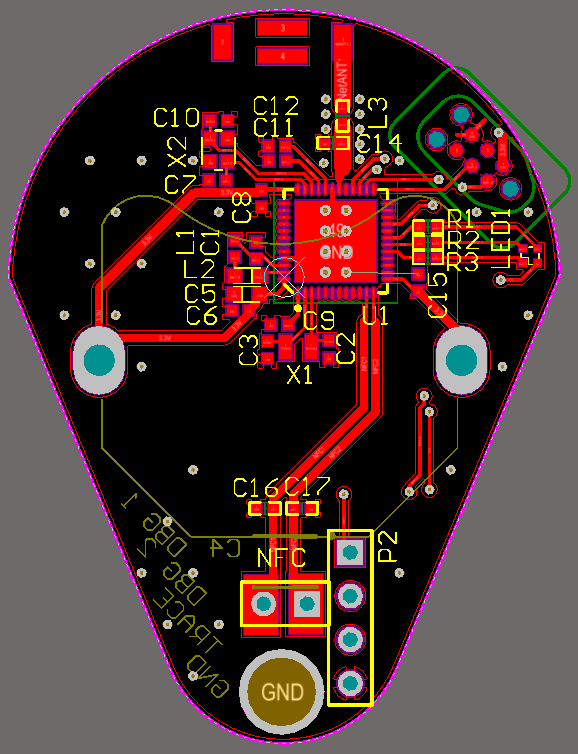
\includegraphics[width=6cm]{img/board_layouts/key_tag_top.png}
	}
	\qquad
	\subfloat[Wizualizacja górnej warstwy płytki]{
		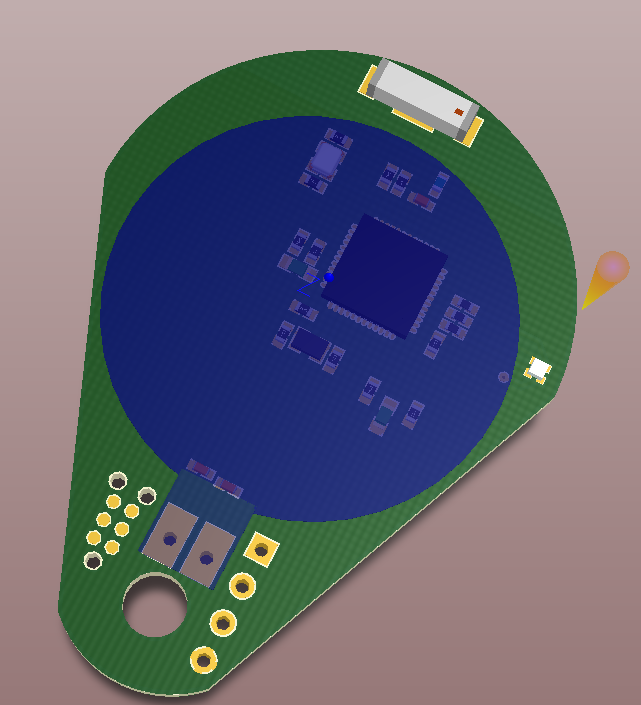
\includegraphics[width=7.1cm]{img/board_layouts/key_tag_visualization_top.png}
	}
	
	\caption{Wygląd górnej warstwy płytki urządzenia dezaktywującego oraz jej wizualizacja}
	\label{fig:image_key_tag_top_board}
\end{figure}

\begin{figure}[H]
\centering
	\subfloat[Wygląd dolnej warstwy płytki]
	{
		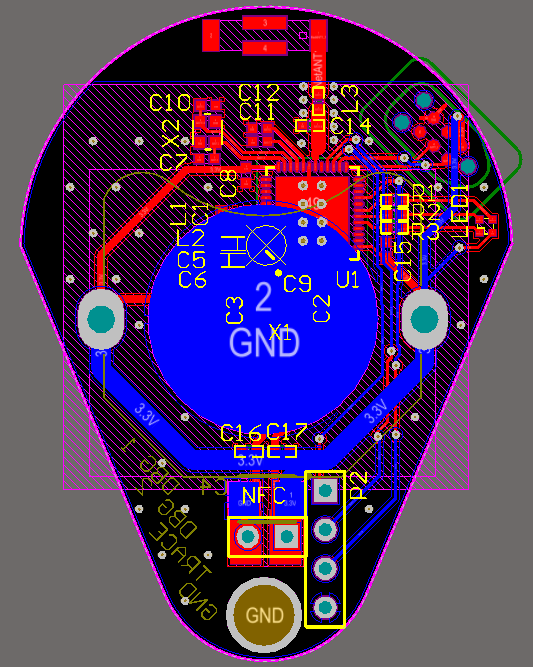
\includegraphics[width=6cm]{img/board_layouts/key_tag_bottom.png}
	}
	\qquad
	\subfloat[Wizualizacja dolnej warstwy płytki]
	{
		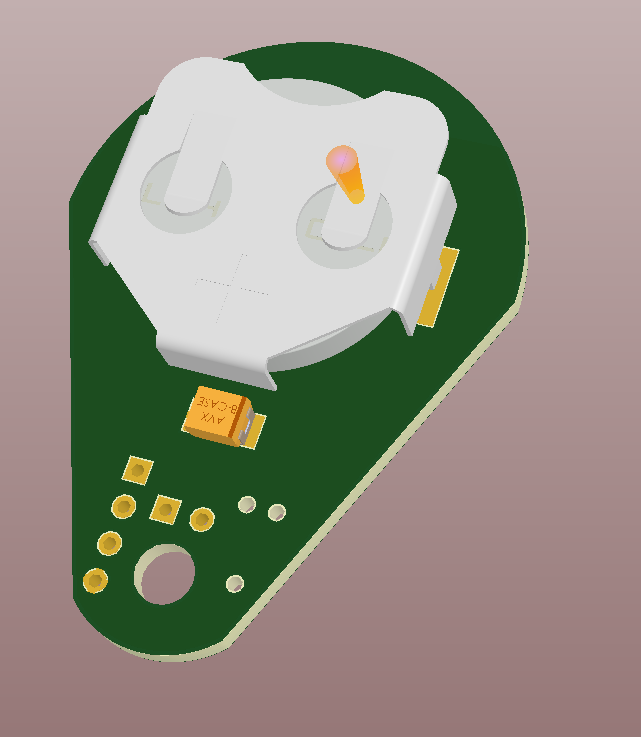
\includegraphics[width=7.1cm]{img/board_layouts/key_tag_visualization_bottom.png}
	}
	
	\caption{Wygląd dolnej warstwy płytki urządzenia dezaktywującego oraz jej wizualizacja}
	\label{fig:image_key_tag_bottom_board}
\end{figure}

\section{Urządzenie lokalizujące}

\begin{figure}[H]
\centering
	\subfloat[Wygląd górnej warstwy płytki]{
		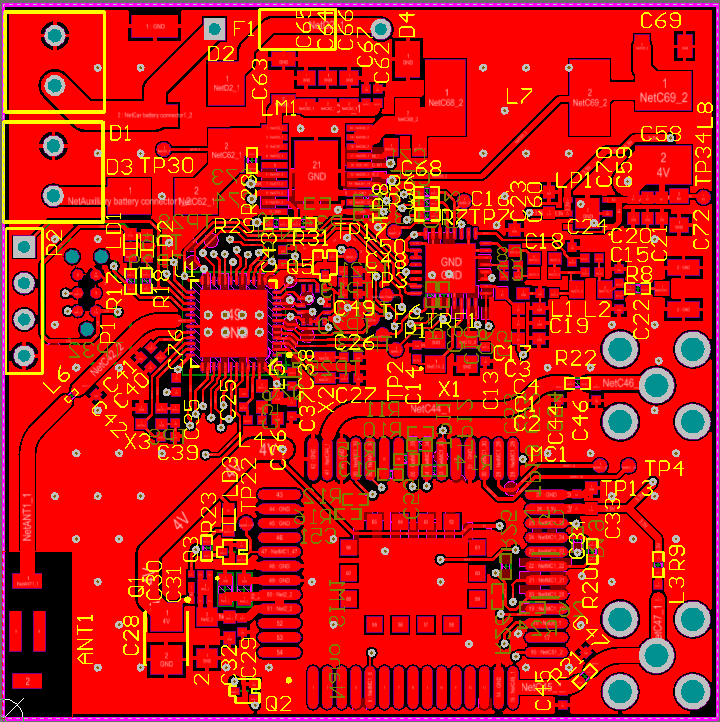
\includegraphics[width=11cm]{img/board_layouts/mainboard_top.png}
	}
	\qquad
	\subfloat[Wizualizacja górnej warstwy płytki]{
		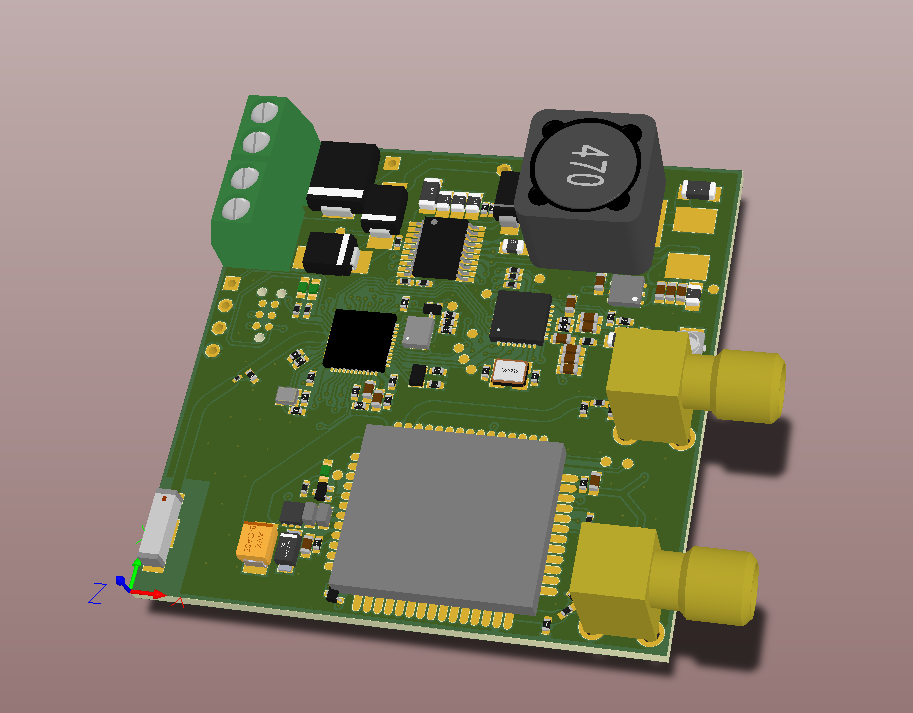
\includegraphics[width=11cm]{img/board_layouts/mainboard_visualization_top.png}
	}
	
	\caption{Wygląd górnej warstwy płytki urządzenia lokalizującego oraz jej wizualizacja}
	\label{fig:image_mainboard_top_board}
\end{figure}

\begin{figure}[H]
\centering
	\subfloat[Wygląd dolnej warstwy płytki]
	{
		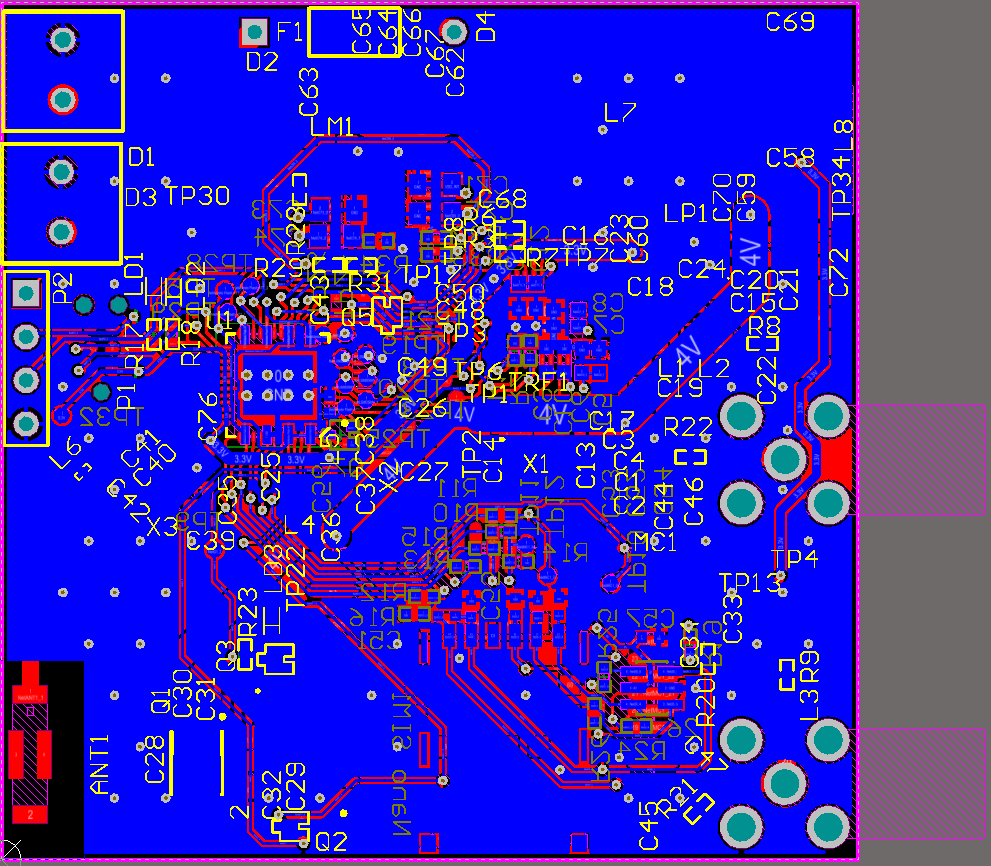
\includegraphics[width=11cm]{img/board_layouts/mainboard_bottom.png}
	}
	\qquad
	\subfloat[Wizualizacja dolnej warstwy płytki]
	{
		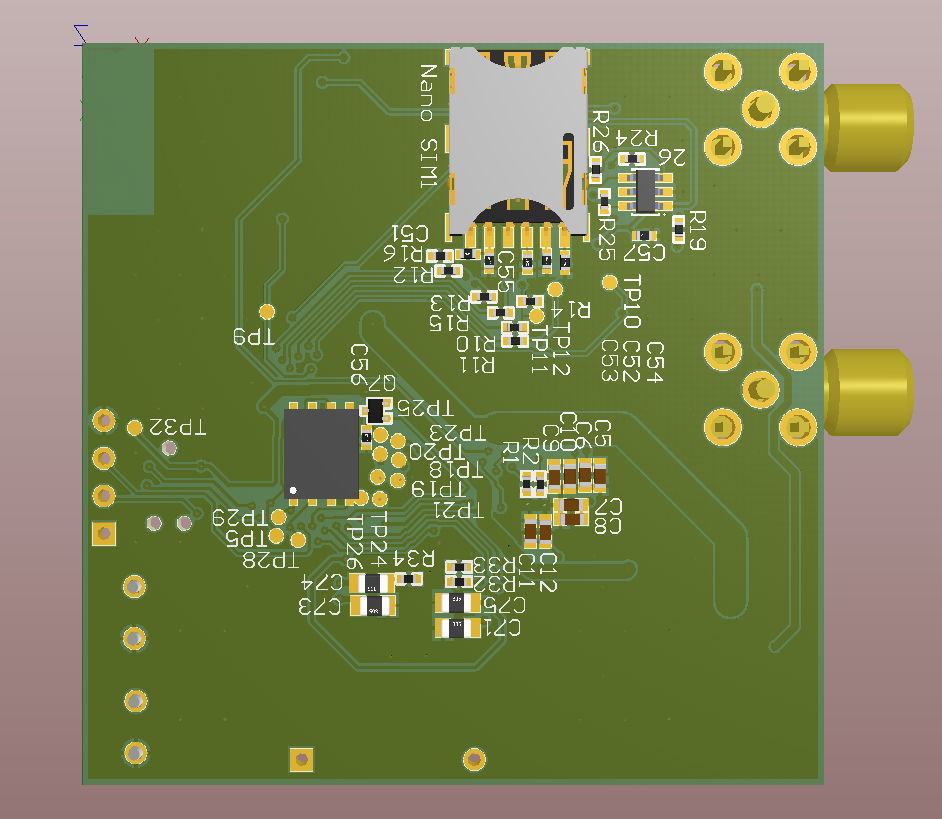
\includegraphics[width=11cm]{img/board_layouts/mainboard_visualization_bottom.png}
	}
	
	\caption{Wygląd dolnej warstwy płytki urządzenia lokalizującego oraz jej wizualizacja}
	\label{fig:image_mainboard_bottom_board}
\end{figure}